%%%%%%%%%%%%%%%%%%%%%%%%%%%%%%%%%%%%%%%%%%%%%%%%%%%%%%%%%%%%%%%%%%%
% Notes (JMH Mar 19, 2014)
% Have added sections on single slit, diffraction limit, and grating
% Still need problems on grating (can be closely modeled on Wolfson problems)
% An example calculation for a diffraction grating
%%%%%%%%%%%%%%%%%%%%%%%%%%%%%%%%%%%%%%%%%%%%%%%%%%%%%%%%%%%%%%%%%%%

\chapter[Phasor Diagrams]{Phasors, Phasor Diagrams, and Wave Interference}
\label{chapter:phasors}
%\setcounter{ex}{0}

\section{Introduction}
\label{sec:phasors_intro}

No, they're not little hand-held devices that can stun and kill
unsuspecting aliens. At least, those aren't the ones we're talking
about here. Phasors provide a way to represent oscillating motion
graphically, and once you understand them a little, they provide for
rather intuitive and straightforward way to handle wave interference
problems.

\section{A Phasor Diagram for a Single Oscillation}
\label{sec:phasor_single}

\begin{figure}\begin{center}
 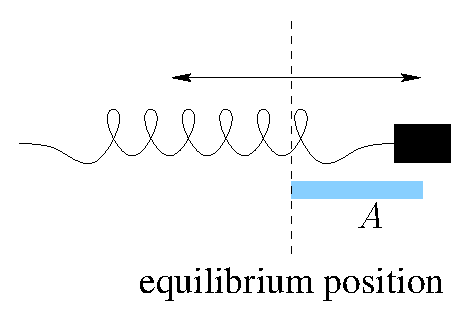
\includegraphics[width=2.0truein]{phasors/phasor01} 
\caption{\label{fig:phasor01} Mass on a spring.}
\end{center}
\end{figure}


Consider a simple oscillating system, like a mass on a spring moving
back and forth on a frictionless horizontal surface.
We can write an expression for the displacement of the mass as follows:
\begin{equation}
x(t) = A\cos{(\omega t)},
\end{equation} 
where $A$ is the amplitude of the oscillation, and $\omega$ is the
angular frequency in units of rad/s. That means that $A$ is
the value of the largest deviation (plus or minus) of the mass from
its equilibrium position, and the value of $\omega$ governs the time it
takes for the mass to complete one oscillation (recall that the period
of the oscillation, $T = 2\pi/\omega$, so a small $\omega$
means a long period while a large $\omega$ means a short period).
Together, $A$ and $\omega$ completely define the oscillation.


We can represent these two quantities, and therefore the oscillation
itself, with a phasor diagram. A phasor is nothing more than a vector
with magnitude $A$ that {\em rotates} with angular velocity $\omega$. The
concept of a rotating vector is a little strange, but it works out really
well for oscillations.  For the oscillation defined above, $x(0) = A$
since $\cos{(0)} = 1$. We can represent the oscillation at this time
with a phasor of length $A$ that lies on the horizontal axis, as seen
in Fig.~\ref{fig:phasor02}.

\begin{figure}\begin{center}
 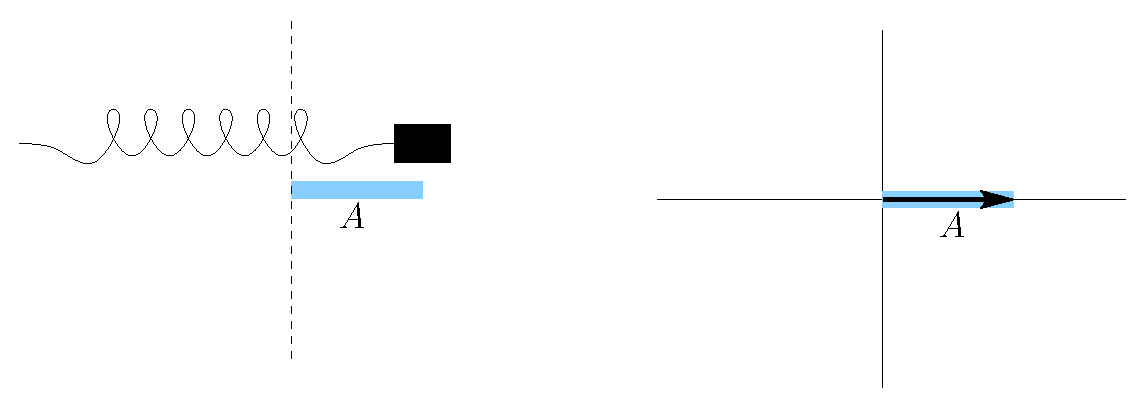
\includegraphics[width=4.0truein]{phasors/phasor02} 
\caption{\label{fig:phasor02}Oscillator and phasor at time $t=0$.}
\end{center}
\end{figure}

Not very interesting yet, I know, but here's the cool part: let time
advance.  As time passes, the mass moves back toward its equilibrium
position. At the same time, the phasor rotates in the counterclockwise
direction. The phasor's magnitude doesn't change, but the projection
of the phasor onto the horizontal axis (i.e., the horizontal
component of the vector describing the phasor) gets smaller, as 
shown in Fig.~\ref{fig:phasor03}.

\begin{figure}\begin{center}
 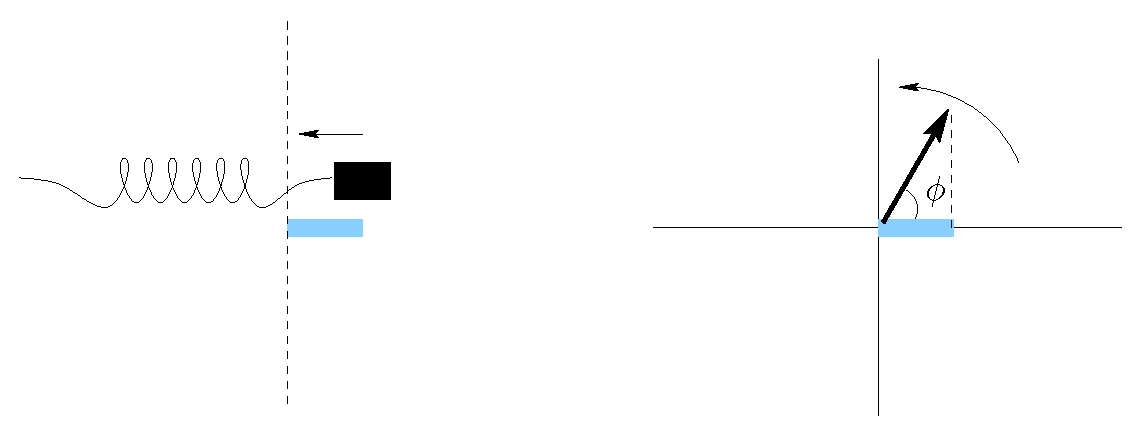
\includegraphics[width=4.0truein]{phasors/phasor03} 
\caption{\label{fig:phasor03}Oscillator and phasor a little bit later.}
\end{center}
\end{figure}

\begin{figure}\begin{center}
 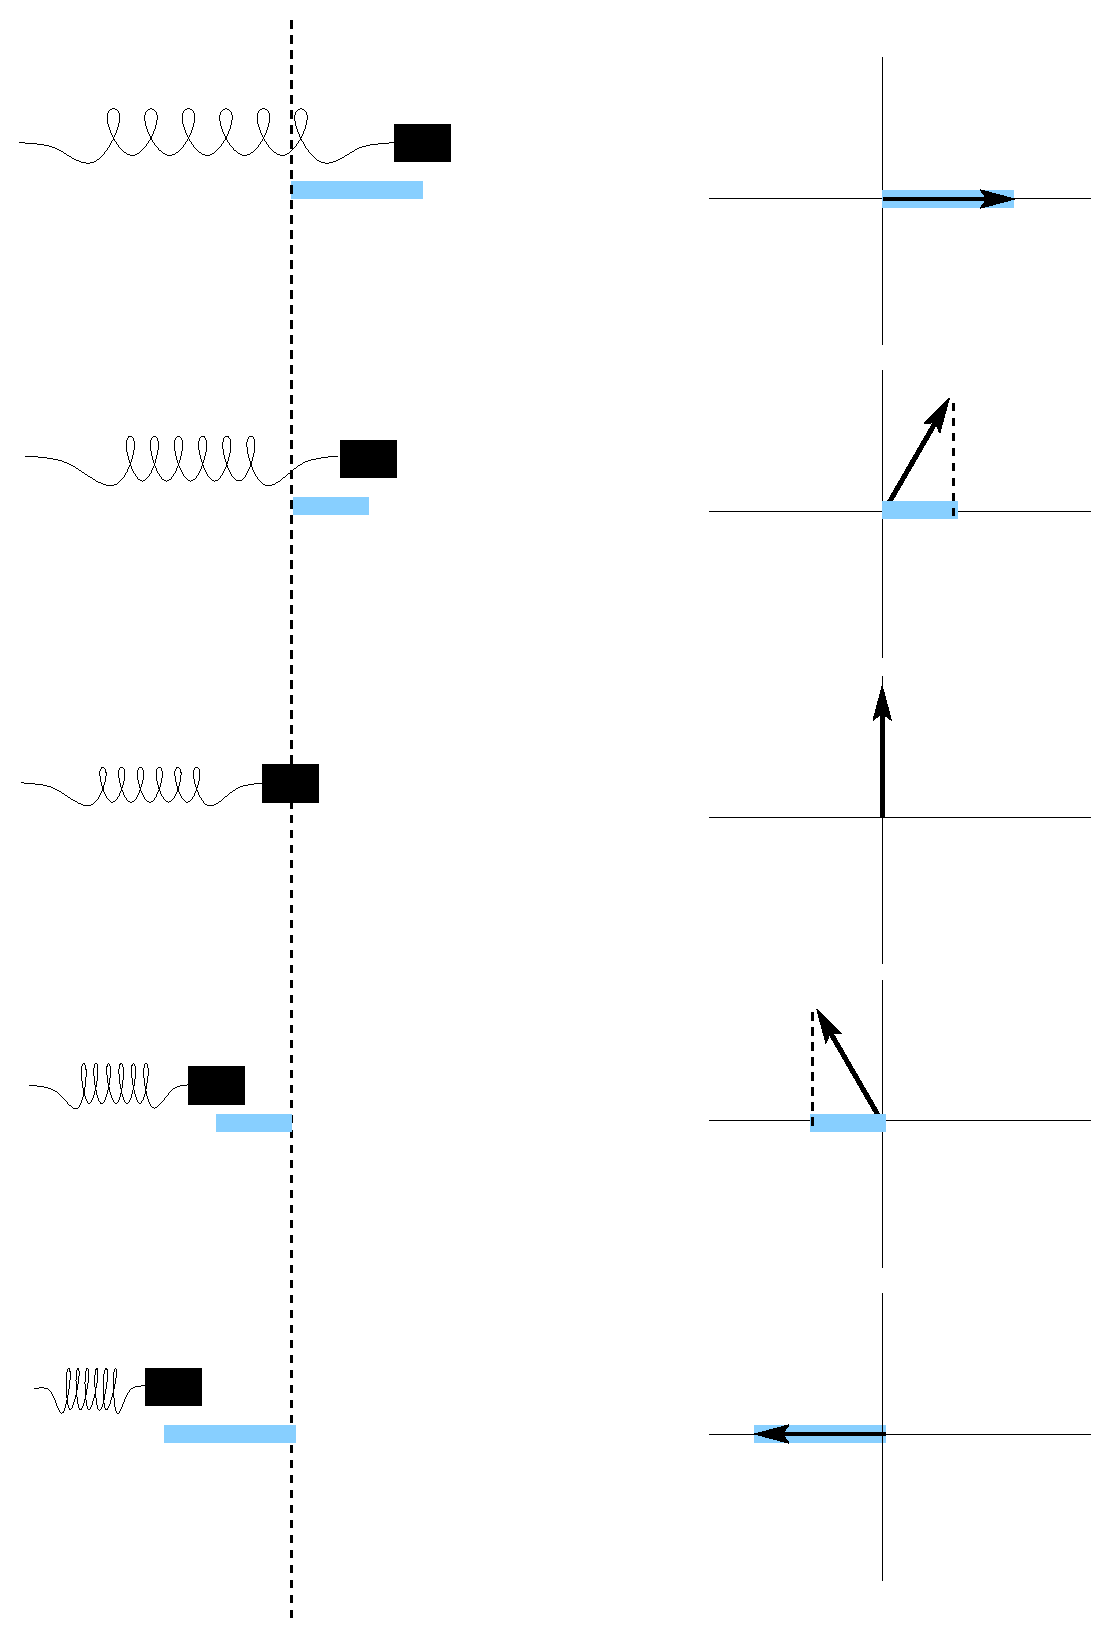
\includegraphics[width=4.0truein]{phasors/phasor04} 
\end{center}\caption{\label{fig:phasor04}Time evolution of the oscillator
and corresponding phasor.}
\end{figure}


Now if $\phi = \omega t$ in the phasor diagram, then the projection of
the phasor on the horizontal axis is $A\cos{(\phi)} = A\cos{(\omega
  t)}$, and that's precisely the expression for the displacement of
the mass at time $t$. This means that if the phasor rotates with
angular velocity $\omega$ and starts in the horizontal position at $t
= 0$, its projection onto the horizontal axis will always describe the
displacement of the oscillation, as seen in Fig.~\ref{fig:phasor04}.


Note that the phasor does not change length; rather, it's just the
projection of the phasor onto the horizontal axis that changes to
describe the oscillation's changing displacement.  This diagram should
also give you a better idea of why we talk about ``angular frequency''
for oscillations. We're matching up the frequency of the oscillation
with the angular velocity of the rotating phasor.

%%\newpage
\begin{example}{A Day at the Beach.} 
\label{example1}
Imagine you're at the beach and you walk into the surf
until you're waist-deep in the water. You feel the waves passing by
you, and you realize that you can express the change in the level of
the water at your location with the expression
\begin{equation}
y(t) = A\cos{(\omega t)},
\end{equation} 
where $A = 20\units{cm}$ and $\omega = \frac{\pi}{3}\units{rad/s}$.
Draw a phasor diagram to depict the level of the water at time
$t = 3\units{s}$.
%\solution
\begin{solution}
The phasor describing this oscillation will have magnitude $A = 20\units{cm}$,
so we need a vector of that length. At time $t = 3\units{s}$, the
phasor will have rotated so that
\begin{equation}
\phi (t) = \omega t = \frac{\pi}{3}\times 3 = \pi\units{rad}. 
\end{equation}
The phasor diagram is illustrated in Fig.~\ref{fig:phasor05}. 
\noindent The projection of the phasor onto the horizontal axis is
$-20\units{cm}$, so at this time, the wave height is at a minimum
(i.e., a trough).

\begin{figure}
\begin{center}
 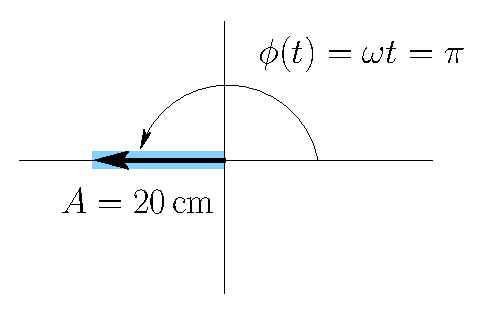
\includegraphics[width=2.5truein]{phasors/phasor05} 
\caption{Phasor diagram for Example~\ref{example1}.
\label{fig:phasor05}}
\end{center}
\end{figure}


{\em Important Note:} Even though this problem is about an oscillation
in the vertical direction, I still measure the displacement of the
oscillation by the projection of the phasor onto the {\em horizontal}
axis. There is no $x$-  or $y$-axis on a phasor diagram, so don't go
and try to match up the orientation of the oscillation with the phasor
diagram.
\end{solution}
\end{example}

%\newpage

\begin{exampleb}{Alarm Bells.} 
\label{example2}
A fire alarm goes off in your dorm. You run outside and stand in the 
cold weather waiting for the fire department to
arrive and turn off the alarm (it's yet another false alarm). While
you're waiting, you get out your pocket oscilloscope and measure the
change in density of the air at your location due to the compression
from the sound waves from the fire alarm. You measure the density
change $\Delta \rho(t)$ to be described by the following expression:
\begin{equation}
\Delta \rho(t) = A\cos{\left(\omega t + \phi_0\right)},
\end{equation} 
where $A = 0.012\units{kg/m$^3$}$, $\omega =5000\pi\units{rad/s}$, 
and $\phi_0 = \frac{\pi}{4}$. You decide to draw a phasor diagram 
describing the density at time $t= 0.1\units{ms}$.
%\solution
\begin{solution}
This problem is a little trickier because of the non-zero $\phi_0$
inside the cosine. Conceptually, it means that when you decided to
define time $t=0$, the oscillation wasn't at a maximum. Instead, at
time $t=0$,
\begin{equation}
\Delta \rho(t) = A\cos{(\phi_0)} 
                  = 0.012\, \cos{\left(\frac{\pi}{4}\right)}
                  = 0.0085\units{kg/m$^3$}.
\end{equation}
\begin{figure}[b]
\begin{center}
 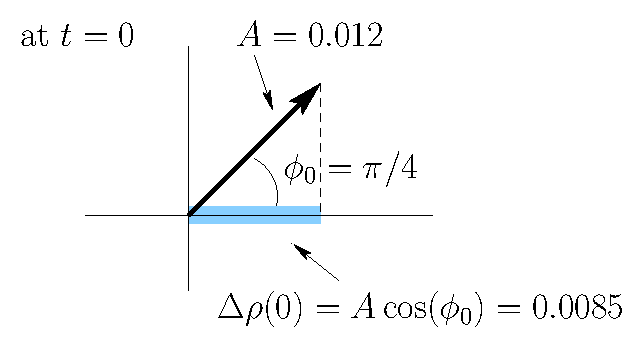
\includegraphics[width=2.75truein]{phasors/phasor06} 
\caption{\label{fig:phasor06}Phasor corresponding to an oscillator
with a phase shift.}
\end{center}
\end{figure}
There's nothing wrong with this, but it will affect how we draw our
phasor diagram. The amplitude of the oscillation is %still 
$A = 0.012\units{kg/m$^3$}$, so that must be the length of our phasor.
However, if the projection of this phasor onto the horizontal axis at
time $t = 0$ is to be $0.0085\units{kg/m$^3$}$, then the phasor must
be rotated. By how much? By $\phi_0$ (see Fig.~\ref{fig:phasor06}).

Fig.~\ref{fig:phasor06} is the ``starting point'' for our phasor diagram. To
produce the phasor diagram for $t = 0.1\units{ms}$, we need to let
this phasor rotate for that time interval. It will rotate by
\begin{equation}
\Delta \phi(t) = \omega t = 5000\pi\times 0.0001 = \frac{\pi}{2}
\end{equation} 
{\em from the starting point} of $\phi_0 = \frac{\pi}{4}$.
So our phasor diagram will look like Fig.~\ref{fig:phasor07}. %this:

\begin{figure}\begin{center}
 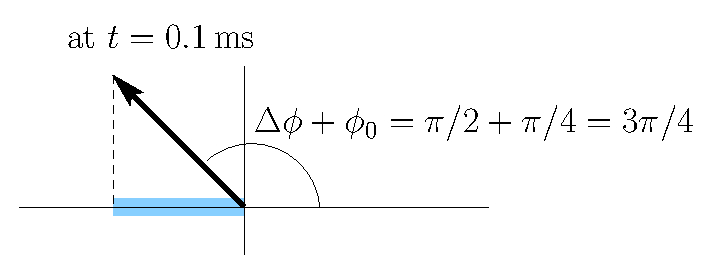
\includegraphics[width=2.5truein]{phasors/phasor07} 
\caption{\label{fig:phasor07}Phasor diagram of oscillator in
Example~\ref{example2} at $t=0.1$}
\end{center}
\end{figure}

The projection of the phasor at this time is
\begin{equation}
A\cos{\left(\frac{3\pi}{4}\right)} = -0.0085\units{kg/m$^3$}. 
\end{equation}
That's the same value we get from the algebraic expression for 
$\Delta \rho (t)$:
\begin{eqnarray}
\Delta \rho (t) & = & A \cos{\left( \omega t + \phi_0\right)}\nonumber\\
               & = & 0.012\, \cos{\left(5000\pi\times 0.1 
                    + \frac{\pi}{4}\right)} \nonumber\\
               & = & 0.012\, \cos{\left(\frac{3\pi}{4}\right)}\nonumber\\
               & = &  -0.0085\units{kg/m$^3$}.
\end{eqnarray}
The change in density at this moment is negative, so the density is
lower than its equilibrium value due to the passing sound wave.
\end{solution}
\end{exampleb}


\section{Phasors as Complex Numbers}
\label{sec:phasor_complex_notation}

You may have encountered complex numbers in your math classes.
Recall that a complex number $z$ can be written as
\begin{equation}
z = a + ib
\end{equation}
with $a$ and $b$ real numbers, and that $i$ is the imaginary unit, 
$i = \sqrt{-1}$.  Here $a$ is called the \textit{real part} of  $z$ 
[written $\mbox{Re}(z)$], while $b$ is called the \textit{imaginary part} 
of $z$ [written $\mbox{Im}(z)$].

It's easy to represent a complex number  graphically.  Just plot the 
real part complex number along the horizontal, or real axis, 
and the imaginary part along the vertical, or imaginary axis,
as shown in Fig.~\ref{fig:complexPlane}.

\begin{figure}\begin{center}
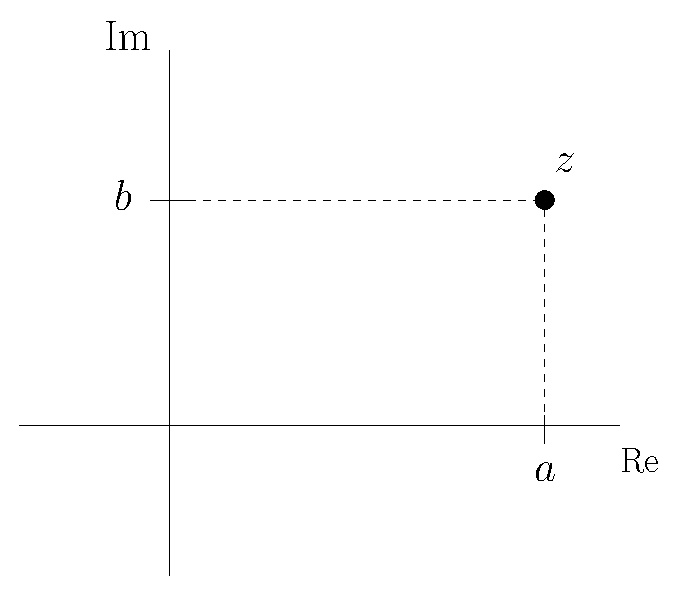
\includegraphics[width=2.2in]{phasors/complex_plane}  
\caption{\label{fig:complexPlane} A complex number can be represented
graphically as a point in the complex plane.}
\end{center}
\end{figure}

The length of the diagonal line from the origin to the point representing
the complex number $z$ is the \textit{magnitude} of $z$, and corresponds
the amplitude of the oscillation $A$, and the angle with respect to the 
positive real axis corresponds to the phase angle $\phi$, as shown in 
Fig.~\ref{fig:complexPhasor}, which is really just a phasor diagram!
\begin{figure}[b]
\begin{center}
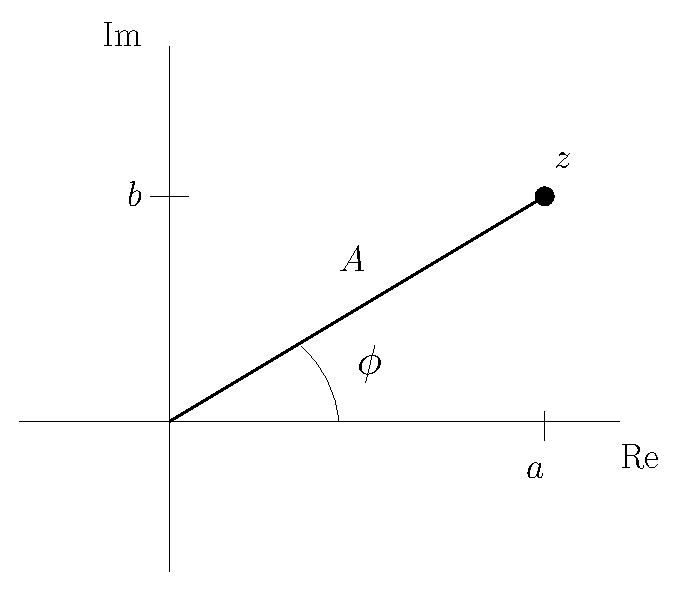
\includegraphics[width=2.2in]{phasors/complex_phasor}  
\caption{\label{fig:complexPhasor}Phasors correspond to complex numbers.}
\end{center}
\end{figure}

Applying simple trig to the diagram gives 
\begin{equation}
a = \mbox{Re}(z) = A \cos\phi\hspace{0.5in}b = \mbox{Im}(z) = A\sin\phi.
\end{equation} 
It is the real part of the complex number that corresponds to the 
physical oscillation,  but using the complex representation actually 
simplifies many calculations.  

The connection to phasors gets even stronger when we make use of the 
Euler identity
\begin{equation}
e^{i\phi} = \cos\phi + i\sin\phi,
\label{eq:euler}
\end{equation}
so that
\begin{eqnarray}
z = a + ib &=& A\cos\phi + i A\sin\phi \nonumber \\
	   &=& A(\cos\phi + i\sin\phi)  \nonumber \\
  	   &=& Ae^{i\phi}.
\end{eqnarray}
Thus, if we have an oscillation represented in complex exponential form,
we can immediately draw its phasor picture:  Make an arrow of length
$A$ at angle $\phi$ from the real (horizontal) axis.

\begin{example}{Another Day at the Beach.}  
\label{example3}
The change in water level at your location is now represented with
the following complex function (whose real part is the actual water
height):
\begin{equation}
y(t) = 25 \, e^{i(\pi/4\, t + \pi/2)},
\end{equation}
with $y$ in cm and $t$ in sec. 
Draw a phasor diagram to depict the level of the water at $t = 2$, 3 and 
$4\units{s}$.
%\solution
\begin{solution}
Draw the real and imaginary axes.  Starting at the real axis, 
go counterclockwise for $\pi/2$ radians (the phase constant $\phi_0$).  
Then keep going counterclockwise $\pi/4$ radians for each second of 
elapsed time.  The phasors are shown in Fig.~\ref{fig:phasorRotation}.

\begin{figure}
\begin{center}
 \scalebox{0.6}{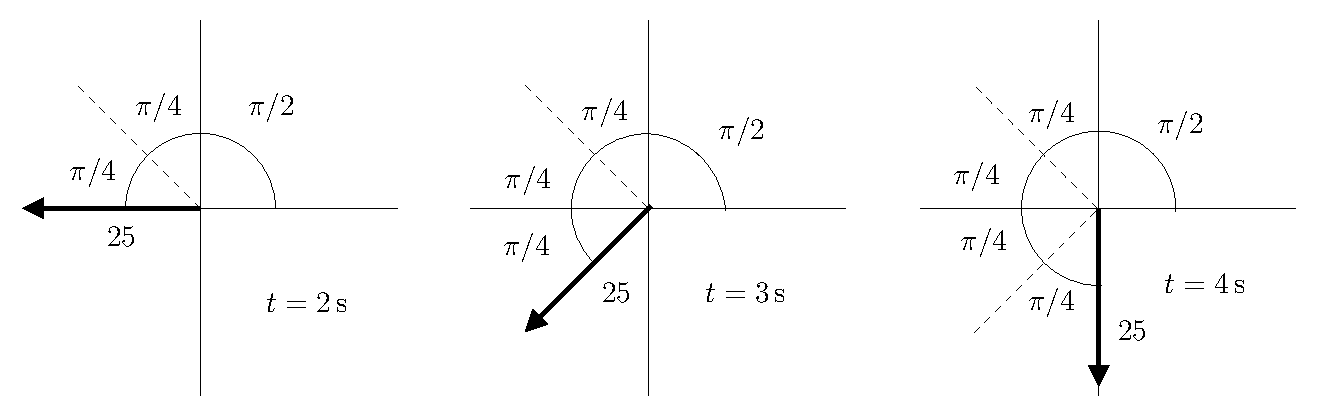
\includegraphics{phasors/phasor_rotation}}  
\caption{\label{fig:phasorRotation}Phasors for the water level in 
Example~\ref{example3} at times $t=2\units{s}$, $t=3\units{s}$, and 
$t=4\units{s}$.}
\end{center}
\end{figure}
To find actual water levels, take the real part (the horizontal projection).  
The water levels are thus   
\begin{eqnarray}
&&\mbox{at $t=2\units{s}$}: \hspace{0.5in}-25\units{cm}\nonumber \\
&&\mbox{at $t=3\units{s}$}: \hspace{0.5in}-25\cos(\pi/4)= 
  -\frac{25}{\sqrt{2}}\simeq-17.7\units{cm}\nonumber\\ 
&&\mbox{at $t=4\units{s}$}:\hspace{0.5in}0\nonumber
\end{eqnarray}
\end{solution}
\end{example}

\section{Adding Phasors}
\label{sec:adding_phasors}

\begin{figure}[b]
\begin{center}
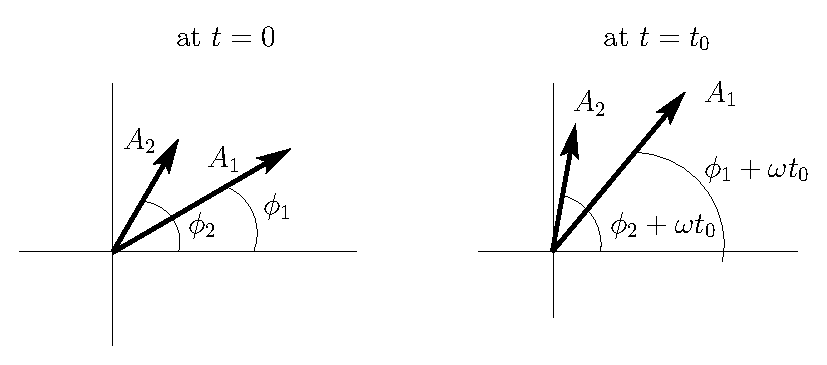
\includegraphics[width=4.2truein]{phasors/phasor08} 
\caption{\label{fig:phasor08}Phasor diagram showing separate phasors 
for oscillations $y_1$ and $y_2$ rotating together with the 
same angular frequency.}
\end{center}
\end{figure}
%

The power and utility of the phasor representation really show up
when combining oscillations. Consider two oscillations, both with the
same angular frequency $\omega$, but with different amplitudes and
phases:
\begin{equation}
y_1(t) = A_1\cos{(\omega t + \phi_1)}\quad \text{and} \quad
y_2(t) = A_2\cos{(\omega t + \phi_2)}.  
\end{equation}
The superposition of these two oscillations, $y_{\rm tot} = y_1 + y_2$,
will be sinusoidal with the same angular frequency $\omega$, 
but it is very messy to calculate the new amplitude and phase shift  
algebraically; it is actually much simpler
using the complex phasor method. Because the oscillation's have 
the same frequency, the phasors rotate together as time passes,
as illustrated in Fig.~\ref{fig:phasor08}.  That is, the angle
between the phasors will always be $\Delta\phi = \phi_2-\phi_1$.

%\begin{figure}\begin{center}
% 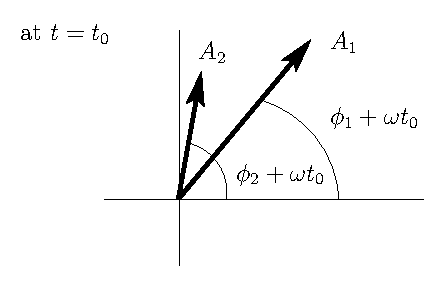
\includegraphics[width=2.4truein]{phasors/phasor08a} 
%\caption{\label{fig:phasor08a}Phasor diagram
%showing phasors for oscillations $y_1$ and $y_2$ at a later time $t=t_0$.
%}
%\end{center}
%\end{figure}


The resultant phasor, with its own amplitude and phase, is illustrated
in Fig.~\ref{fig:phasor09}.  We can determine the amplitude and phase
of the resultant phasor by adding the two input phasors the same way we
add vectors.  The amplitude of the resultant will be less than the sum
of the two original phasor amplitudes (unless $\Delta\phi = 0$) and the
phase of the resultant will be something between the phases of the two
original phasors.

\begin{figure}
\begin{center}
 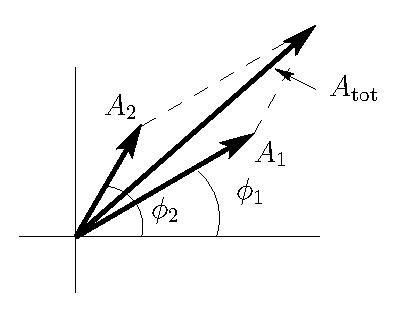
\includegraphics[width=2.0truein]{phasors/phasor09} 
\caption{\label{fig:phasor09}The combined oscillation is described by 
a phasor that is the vector sum of the two separate phasors.}
\end{center}
\end{figure}

\begin{example}{Rock Your Boat.} 
\label{example4}
You're sitting in a boat in the middle of a calm lake. Suddenly a motor
boat drives by, producing waves that would oscillate your boat up and
down as follows:
\begin{equation}
y_1(t) = A_1\cos{(\omega t + \phi_1)}, 
\end{equation}
where $A_1 = 25\units{cm}$, $\omega = \frac{2\pi}{3}$, and
$\phi_1 = \frac{\pi}{6}$. At the same time, another motor boat drives
by, producing waves that would oscillate your boat up and down as follows:
\begin{equation}
y_2(t) = A_2\cos{(\omega t + \phi_2)}, 
\end{equation}
where $A_2 = 15\units{cm}$, $\omega = \frac{2\pi}{3}$, and
$\phi_1 = \frac{\pi}{3}$. However, since both waves act on the boat
simultaneously, the actual oscillation of your boat is the
superposition of these two waves. How much does your boat move up and
down as a result of the combination of these waves?
%\solution
\begin{solution}
The phasor diagram for these two separate oscillations %looks like this:
is shown in Fig.~\ref{fig:phasor10}.
The resultant phasor can be determined from the vector addition of the
phasors shown in Fig.~\ref{fig:phasor11}.

\renewcommand{\arraystretch}{2.0}
\begin{center}
\begin{tabular}{|c|c|c|}\hline
\quad Phasor\quad &
\quad real part (horizontal) \quad &
\quad imaginary part (vertical) \quad \\ 
\hline\hline
1      & $25\cos\left(\frac{\pi}{6}\right) = 21.6$ 
       & $25\sin\left(\frac{\pi}{6}\right) = 12.5$ \\ \hline 
2      & $15\cos\left(\frac{\pi}{3}\right) =7.5$ 
       & $15\sin\left(\frac{\pi}{3}\right) =13.0$ \\
\hline\hline
Total  & $29.1$   & $25.5$ \\
\hline
\end{tabular}
\end{center}
\renewcommand{\arraystretch}{1.0}

\begin{figure}\begin{center}
 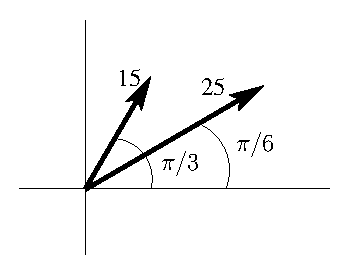
\includegraphics[width=2.0truein]{phasors/phasor10} 
\caption{\label{fig:phasor10}Phasor diagram for 
two water waves in Example~\ref{example4}. }
\end{center}
\end{figure}

\noindent So, the amplitude of the resultant phasor is 
\begin{equation}
A_{\rm tot} = \sqrt{29.1^2 + 25.5^2} =38.7\units{cm}, 
\end{equation} 
and its initial phase is 
\begin{equation}
\phi_{\rm tot} = \tan^{-1}{\left(\frac{25.5}{29.1}\right)} 
                  = 0.72\units{rad}.  
\end{equation} 

\begin{figure}[b]
\begin{center}
 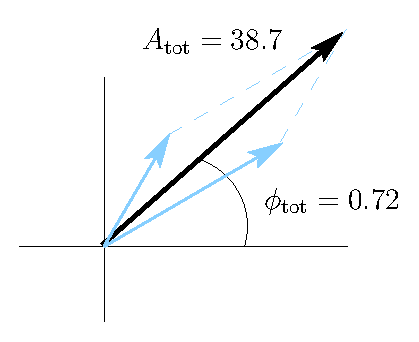
\includegraphics[width=2.0truein]{phasors/phasor11} 
\caption{\label{fig:phasor11}Phasor addition  for 
two water waves in Example~\ref{example4}.}
\end{center}
\end{figure}
We can write the superposition as
\begin{eqnarray*}
 y_{\rm tot}(t) & = & A_{\rm tot}\cos{(\omega t + \phi_{\rm tot})} \\
            & = & 38.7\cos{(\omega t + 0.72)}, \\
\end{eqnarray*}
with $y$ in cm and $t$ in sec.
\end{solution}
\end{example}
\newpage

\begin{exampleb}{Two Towers.} 
\label{exampleTwoTowers}
\begin{figure}\begin{center}
 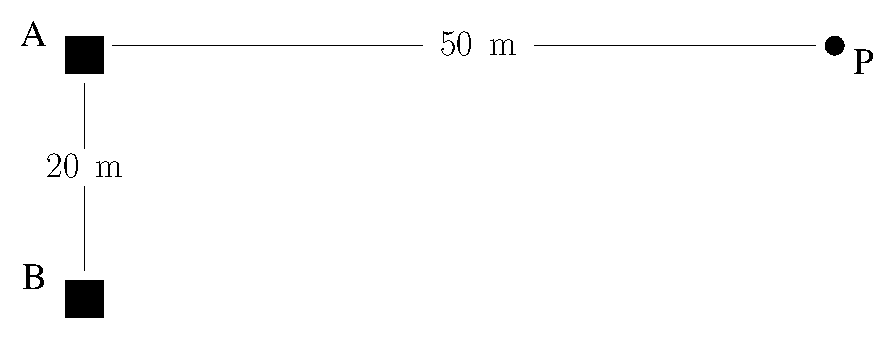
\includegraphics[width=3.0truein]{phasors/phasor12} 
\caption{\label{fig:phasor12}Illustration of radio towers in 
Example~\ref{exampleTwoTowers}.}
\end{center}
\end{figure}
Two radio towers, A and B, separated by $20\units{m}$,
broadcast the same radio signal of wavelength $\lambda =
12\units{m}$. You're standing at the point $P$ indicated in the
figure with your radio wave amplitude meter.
With only tower A broadcasting, you measure a wave amplitude
of 7 (in some unspecified unit).  With only tower B broadcasting, you
measure a wave amplitude of 5. What amplitude do you measure when both
towers are broadcasting?
%\solution
\begin{solution}
Here we're interested in the superposition of the waves from the two
towers. We aren't explicitly given the phase difference between the
wave signals that arrive at $P$ from the two towers, but we can figure
it out because we know the distances from point $P$ to each tower. If
the waves leave the two towers in phase, they won't necessarily be in
phase when they reach point $P$ because the waves from Tower B have to
travel farther. How much farther? Well, the distance between Tower B
and point $P$ is $\sqrt{50^2 + 20^2} = 53.85\units{m}$, so the waves
from Tower B have to travel $3.85\units{m}$ farther. That means the
waves from Tower A will be $3.85\units{m}$ ahead of the waves from
Tower B.

We can turn that distance difference into a phase difference for the
waves. The path length difference $\Delta r = 3.85\units{m}$ produces
$\frac{3.85}{12} = 0.32$ {\em wavelengths} of difference between the two
waves as they arrive at point $P$.
If the waves from Tower A arrived exactly one wavelength ahead of the
waves from Tower B, the signals would add constructively. The phase
difference would be $2\pi$, and peaks and troughs of the two waves
would be aligned. In this case, however, the waves from Tower A arrive
only $0.32\units{wavelengths}$ ahead of the waves from Tower B.
Consequently, the phase difference $\Delta\phi$ is
\begin{equation}
\Delta\phi = 2\pi \frac{\Delta r}{\lambda} = 2\pi \frac{3.85}{12} 
= 2.0\units{rad}.
\end{equation} 
We can then write expressions for the two oscillations at point $P$ as
follows:
\begin{equation}
y_A(t) = 7\cos{\left(\omega t + 2.0\right)} \quad\quad
 y_B(t) = 5\cos{\left(\omega t\right)}.
\end{equation}
Why did I pick zero initial phase for the signal from Tower B?
Because I could. In this case (and in most cases we'll deal with),
we're only interested in the phase difference between signals.
Therefore, I can always choose to describe one wave with zero initial
phase, and then put the phase difference into the expression for the
other wave. With one phasor on the horizontal axis, the phasor
addition is just easier.

Now we can construct a phasor diagram for the two oscillations, shown
in Fig.~\ref{fig:phasor13}.

\begin{figure}\begin{center}
 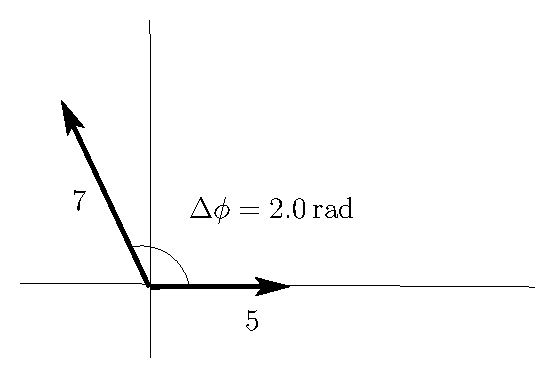
\includegraphics[width=2.4truein]{phasors/phasor13} 
\caption{\label{fig:phasor13}Phasor diagram for radio waves in 
Example \ref{exampleTwoTowers}.}
\end{center}
\end{figure}

Once again, the resultant phasor can be determined from the vector
addition of the phasors.

\renewcommand{\arraystretch}{2.0}
\begin{center}
\begin{tabular}{|c|c|c|}\hline
\quad Phasor\quad\mbox{} &
\quad real part (horizontal) \quad \mbox{}&
\quad imaginary part (vertical) \quad\mbox{} \\ 
\hline\hline
1      & $5\cos{\left(0\right)}=5$ & $5\sin{\left(0\right)}=0$ \\
\hline
2      & $7\cos{\left(2.0\right)}=-2.9$ & $7\sin{\left(2.0\right)}=6.4$ \\
\hline\hline
Total  & $2.1$   & $6.4$ \\
\hline
\end{tabular}
\end{center}
\renewcommand{\arraystretch}{1.0}
\vspace{0.08in}

So, the amplitude of the resultant phasor is 
\begin{equation}
A_{\rm tot} = \sqrt{2.1^2 + 6.4^2} = 6.7,
\end{equation}
and its initial phase is
\begin{equation}
\phi_{\rm tot} = \tan^{-1}{\left(\frac{6.4}{2.1}\right)} 
      = 1.25\units{rad},
\end{equation} 
and we can thus write the superposed oscillation as
\begin{equation}
y_{\rm tot}(t) = 6.7\cos{(\omega t + 1.25)}. 
\end{equation}
\end{solution}
\end{exampleb}

\section[Multi-Source Interference]{Phasor Diagrams for Multiple Source Interference}
\label{sec:phasors_multiple_source}

Sometimes, more than two waves will interfere at a single point. In
these cases, the total amplitude of the combined oscillation will be
the superposition of all of the incident waves. The phasor addition
technique can be used to calculate the total amplitude in these
complicated cases. Consider, for example, three oscillations, all with
the same angular frequency $\omega$, but with different amplitudes and
phases:

\begin{eqnarray*}
y_1(t) & = & A_1\cos{(\omega t + \phi_1)}, \\
y_2(t) & = & A_2\cos{(\omega t + \phi_2)}, \ {\rm and} \\
y_3(t) & = & A_3\cos{(\omega t + \phi_3)}.
\end{eqnarray*}
These three oscillations can be expressed graphically, as shown in 
Fig.~\ref{fig:phasor15},
 and their superposition, $y_{\rm tot} = y_1 + y_2 + y_3$, can
be determined from vector addition of the three phasors.


\begin{figure}\begin{center}
 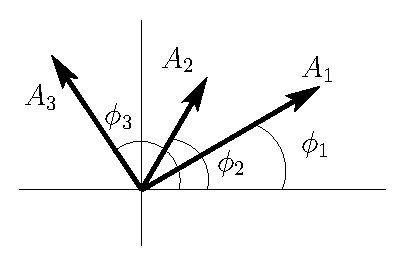
\includegraphics[width=2.4truein]{phasors/phasor15} 
\caption{\label{fig:phasor15}Phasors for the three oscillations $y_1$, $y_2$, 
and $y_3$.}
\end{center}
\end{figure}
%\noindent 

One of the most common multi-source interference problems is an
extension of the two-slit problem considered in class. Imagine a light
source passing through a screen containing not two but {\em three}
slits, each separated from its neighbor by a distance $d$, as shown
in Fig.~\ref{fig:phasor16}.
 The interference pattern for this arrangement of slits will
look different from the interference pattern for a two-slit setup.


\begin{figure}\begin{center}
 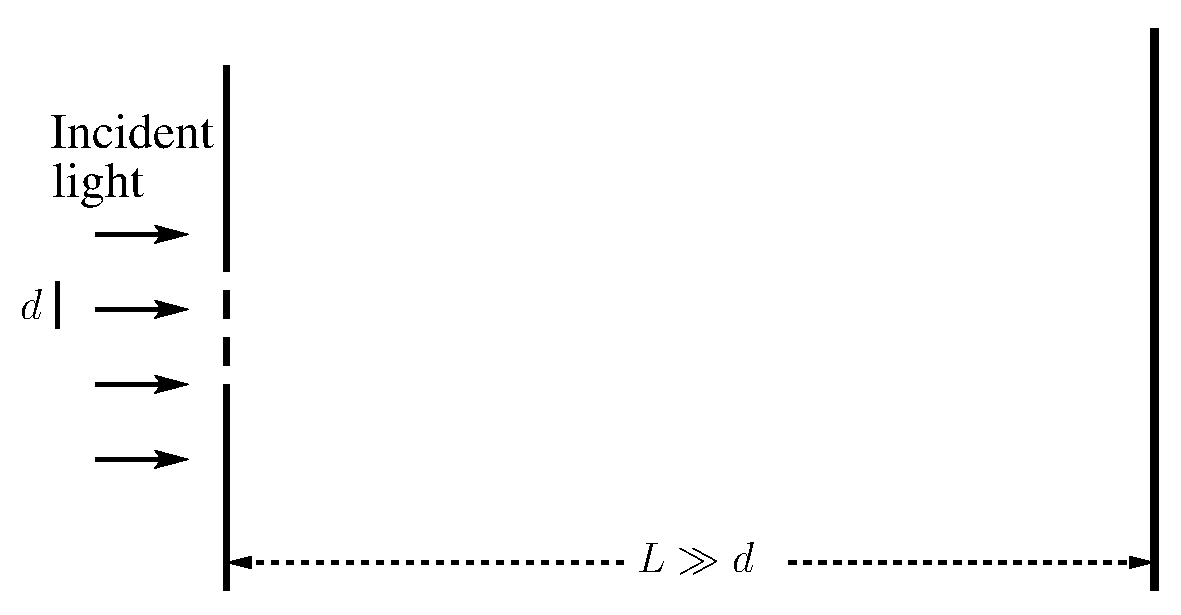
\includegraphics[width=3.0truein]{phasors/phasor16} 
\caption{\label{fig:phasor16}Three closely spaced slits, illuminated straight-on
from the right. The interference pattern is observed on a distant screen to the right.}
\end{center}
\end{figure}



\begin{figure}\begin{center}
 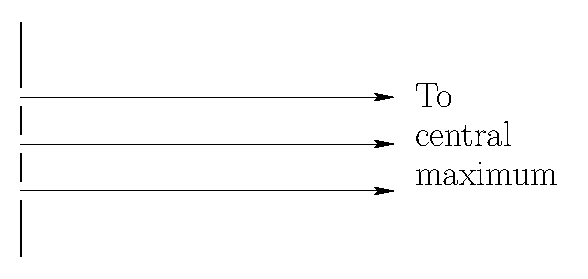
\includegraphics[width=2.0truein]{phasors/phasor17} 
\caption{\label{fig:phasor17}Light rays exiting the three slits
parallel to the normal.}
\end{center}
\end{figure}


If the interference pattern illuminates a screen a distance $L$ from
the slits, where $L\gg d$, then we can assume that the light rays from
each of the slits to any particular point on the screen are parallel.
(This is the same approximation we made in the two-slit case.) For
example, light passing straight through the slits and continuing
straight to the screen produce the central maximum in the interference
pattern, as in Fig.~\ref{fig:phasor17}.
 These rays combine constructively because there's no
difference in the path length for the three light rays, i.e., $\Delta
r = 0$ for all three rays.

Now consider the light rays traveling at an angle $\theta$ to the normal,
as in Fig.~\ref{fig:phasor18}.
 Just as in the two-slit case, these rays do not travel the
same distance to reach the screen. Light from the bottom slit travels
the shortest distance, while light from the middle slit travels an
extra distance $\Delta r_{21}$, and light from the top slit travels
the same amount of extra distance ($\Delta r_{32} = \Delta r_{21}$)
compared to light from the middle slit (Here, I've implicitly labeled
the slits, \#1, 2, and 3 for bottom, middle, and top.).


\begin{figure}\begin{center}
 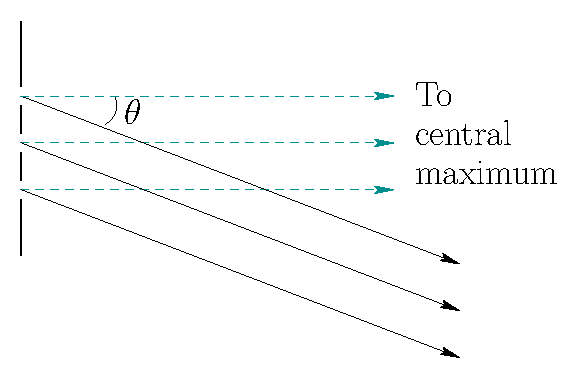
\includegraphics[width=2.0truein]{phasors/phasor18} 
\caption{\label{fig:phasor18}Light rays exiting at an angle $\theta$ to
the normal.}
\end{center}
\end{figure}


\begin{figure}\begin{center}
 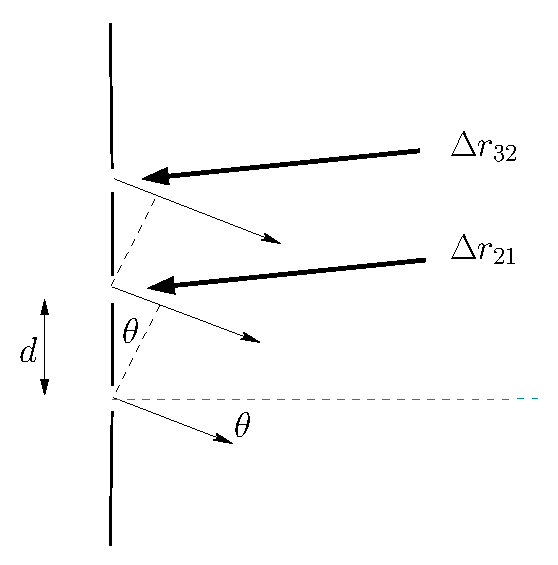
\includegraphics[width=2.0truein]{phasors/phasor19} 
\caption{\label{fig:phasor19}Geometry of path-length difference
between rays from three slits. As for the double slit, the path length
difference for adjacent slits is $d\sin\theta$ if the rays are nearly parallel.}
\end{center}
\end{figure}

From the geometry of the problem (shown in Fig.~\ref{fig:phasor19}), it's clear that $\Delta
r_{32} = \Delta r_{21} = d\sin{\theta}$. We can then calculate the
phase difference between light from adjacent slits,
\begin{equation}
\Delta \phi = 2\pi \frac{\Delta r}{\lambda}
= 2\pi \frac{d\sin{\theta}}{\lambda}.
\end{equation}
With knowledge of the phase difference, we can draw a phasor diagram
and plot phasors for all three light rays, as shown in Fig.~\ref{fig:phasor20}.
We've assumed that the amplitudes of all three phasors
is the same, and  connected the phasors head-to-tail instead of
placing all three with tails at the origin. Note that $\Delta\phi$ is
the phase difference between {\em adjacent} phasors. The total
amplitude of the combined rays is just the vector sum of the phasors:

\begin{figure}
\begin{center}
 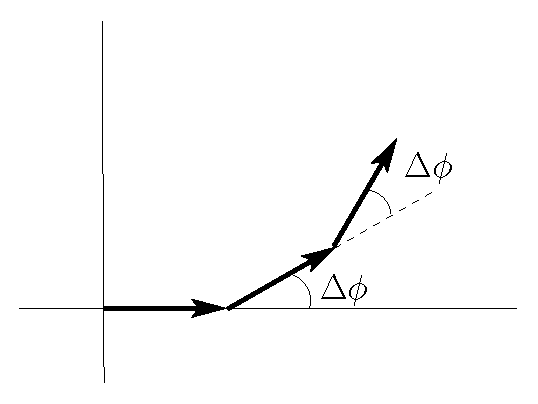
\includegraphics[width=2.0truein]{phasors/phasor20} 
\caption{\label{fig:phasor20}Three phasors, with adjacent phase difference
$\Delta\phi_\text{adj.}$.}
\end{center}
\end{figure}

\begin{figure}
\begin{center}
 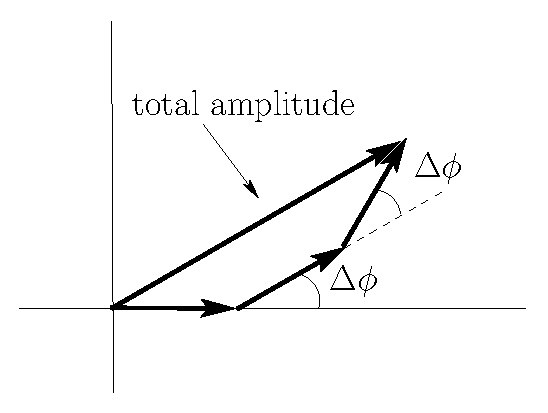
\includegraphics[width=2.0truein]{phasors/phasor21} 
\caption{\label{fig:phasor21}The resultant phasor is the vector sum of the
three phasors corresponding to waves from the three slits.}
\end{center}
\end{figure}

\begin{example}{Combining Three Beams.} 
\label{exampleThreeBeams}
Light of wavelength $\lambda = 478\units{nm}$ passes
through a three-slit system where the slits are separated by a
distance $d = 1.5 \times 10^{-6}\units{m}$, and produces an
interference pattern on a distant screen. What is the amplitude of the
light directed at an angle $\theta = 1.2^\circ$ from the direction to
the central maximum in the interference pattern? Assume that the
amplitude of the light from each slit individually is $A$.
%\solution
\begin{solution}
This is a direct application of the method described above. The phase
difference between adjacent slits is

\begin{eqnarray*}
\Delta \phi & = & 2\pi \frac{\Delta r}{\lambda}\\
            & = & 2\pi \frac{d\sin{\theta}}{\lambda} \\
            & = & 2\pi \frac{1.5 \times 10^{-6}\times \sin{(1.2^\circ)}}
            {478 \times 10^{-9}} \\
            & = & 0.41\units{rad}.\\
\end{eqnarray*}

Therefore, our phasor diagram looks like Fig.~\ref{fig:phasor22}.
To calculate the total amplitude, we again add the phasors as vectors:

\begin{figure}[b]
\begin{center}
 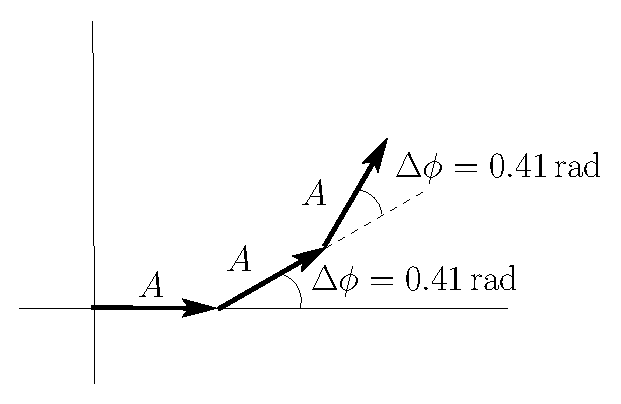
\includegraphics[width=2.4truein]{phasors/phasor22} 
\caption{\label{fig:phasor22}Phasor diagram for Example~\ref{exampleThreeBeams}.}
\end{center}
\end{figure}


\renewcommand{\arraystretch}{2.0}
\begin{center}
\begin{tabular}{|c|c|c|}\hline
\quad Phasor\quad &
\quad real part (horizontal) \quad &
\quad imaginary part (vertical) \quad \\ 
\hline\hline
1      & $A\cos\left(0\right) = A$ & $A\sin\left(0\right) = 0$ \\
\hline
2      & $A\cos\left(0.41\right)= 0.92A$ & $A\sin\left(0.41\right) = 0.40A$ \\
\hline
3      & $A\cos\left(0.82\right)=0.68A$ & $A\sin\left(0.82\right)=0.73A$ \\
\hline
\hline
Total  & $2.6A$   & $1.13A$ \\
\hline
\end{tabular}
\end{center}
\renewcommand{\arraystretch}{1.0}

So the amplitude of the resultant phasor is 
\begin{equation}
A_{\rm tot} = \sqrt{(2.6A)^2 + (1.13A)^2} = 2.83A.
\end{equation}
\end{solution}
\end{example}

\begin{exampleb}{Minimum Light.} 
For the same setup as in the previous example, 
at what angle $\theta$ would you expect to find the first minimum?
%\solution
\begin{solution}
A minimum in the interference pattern will occur when the amplitude of
the resultant phasor is zero, so we need to arrange the three phasors
such that they add to zero. When we had only two phasors, this was
quite easy -- we chose $\Delta \phi = \pi$. In this case, however, we
need to make {\em three} phasors add to zero, and $\Delta \phi = \pi$
won't work (what would a phasor diagram with three phasors, each
differing in phase from its neighbor by $\Delta \phi = \pi$ look like?)

\begin{figure}\begin{center}
 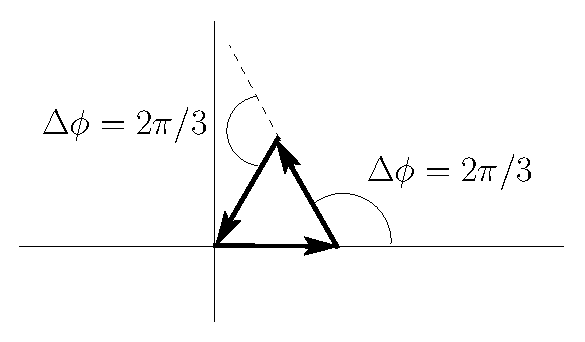
\includegraphics[width=2.4truein]{phasors/phasor23} 
\caption{\label{fig:phasor23}Phasor diagram at the first minimum of the three-slit
interference pattern.}
\end{center}
\end{figure}
 

To get three phasors to add to zero, we need a diagram like
Fig.~\ref{fig:phasor23}, where the phase difference between adjacent
phasors is $\Delta\phi = \frac{2\pi}{3}\units{rad}$. Make sure you
understand why this arrangement yields a total amplitude of zero.

Now that we know the required value for $\Delta\phi$, we can relate
this to the path length difference between adjacent slits:
\begin{equation}
\Delta r = \frac{\Delta\phi}{2\pi} \lambda.
\end{equation} 

Since $\Delta r = d\sin{\theta}$, we can solve for $\sin{\theta}$:
\begin{eqnarray*}
\sin{\theta} & = & \frac{\Delta r}{d} \\
             & = & \frac{\Delta\phi\lambda}{2\pi d} \\
             & = & \frac{2\pi(478 \times 10^{-9})}{6 \pi (1.5 \times 10^{-6})}\\
             & = & 0.106
\end{eqnarray*}
and therefore $\theta = \sin^{-1}{(0.106)} = 6.1^\circ$.


\begin{figure}
\begin{center}
 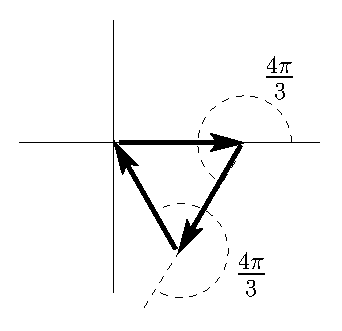
\includegraphics[width=2.0truein]{phasors/phasor24}
\caption{\label{fig:phasor24}Phasor diagram at second minimum of the
 three-slit interference pattern.
}
\end{center}
\end{figure}

There's actually another way to make three phasors add to zero, and
the phasor diagram looks like Fig.~\ref{fig:phasor24}:
In this case, $\Delta\phi = \frac{4\pi}{3}$, and you can show that
this minimum will occur for $\theta = 12.3^\circ$.
\end{solution}
\end{exampleb}

\newpage
\section{Single-Slit Diffraction}
\label{sec:single_slit_diffraction}

\begin{figure}[t]
\begin{center}
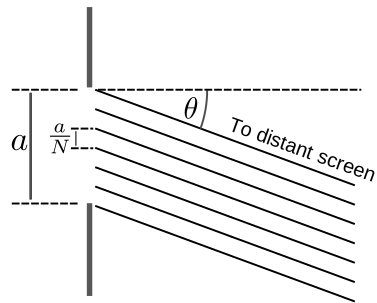
\includegraphics[width=2.5in]{phasors/singleSlitPhases}
\end{center}
\caption{\label{singleSlitPhases}Subdividing a single
slit of width $a$ into $N$ pieces of width $a/N$.}
\end{figure}


We've been assuming that all the slits used to produce diffraction
patterns were very narrow. This meant that the distance from any point
on the slit to a given point on the distant screen was the same. But
what if we have a wide slit?  (By wide, we mean a slit whose width $a$
is comparable to or larger than the wavelength $\lambda$, but still very
small compared with the distance to the screen $L$. ) For such a slit the
light from different parts of the slit may travel different distances
on its way to the screen, and end up with different phase shifts.
This seems like a complicated problem, but fortunately our phasor
techniques are up to the job.

Here's the basic idea: we'll divide the wide slit up into a bunch of
narrow sub-slits.  We'll calculate the phasor corresponding to the
wave from each sub-slit. And we'll add the phasors together to get a
total amplitude.

Specifically, let's call the width of the slit $a$, and divide the
slit into $N$ pieces of width $a/N$
as shown in Fig.~\ref{singleSlitPhases}. We'll keep $N$ a variable, since
we may want to divide the slit into 100 pieces, or 1000, or 10,000, or
even take the limit $N\rightarrow\infty$.  The phase difference
between any two of our adjacent sub-slits is
\begin{equation}
\Delta\phi_{\rm adj.} = \frac{2\pi \Delta r_{\rm adj.}}{\lambda} .
\end{equation}
And since the distance between two adjacent sub-slits is $d=a/N$, 
the adjacent path-length difference is
\begin{equation}
\Delta r_{\rm adj.} = d\sin\theta= \frac{ a}{N} \sin\theta,
\end{equation} 
and the adjacent phase difference is
\begin{equation}
\Delta\phi_{\rm adj.} = \frac{2\pi a}{N\lambda}\sin\theta . 
\end{equation} 
We'll assume
each sub-slit is equally illuminated, so the out-going wave from each
sub-slit has the same amplitude $A$. (Of course, as we divide the slit
into more pieces, the light power in each piece will go down, so $A$
will decrease.  But for a fixed value of $N$ the amplitude $A$ is just
a constant.)

\begin{figure}[t]
\begin{center}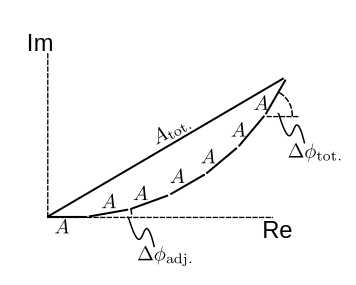
\includegraphics[width=2.5in]{phasors/manySlitPhasorsGeneral}
\end{center}
\caption{\label{manySlitPhasorsGenFig}General phasor diagram for the
single-slit diffraction pattern.}
\end{figure}


We can now draw our phasor diagram. It consists of $N$ equal-length
phasors, each rotated by $\Delta\phi_{\rm adj.} = \frac{2\pi
a}{N\lambda}\sin\theta$ relative to its neighbor, as seen in 
Fig.~\ref{manySlitPhasorsGenFig}.  The final phasor is rotated
by $N$ times $\Delta\phi_{\rm adj.}$, or
\begin{equation}
\Delta\phi_{\rm tot.}=\frac{2\pi a}{\lambda}\sin\theta.
\end{equation}
(Note that this is
the same as the phase difference between the phasor from the top of
the slit and phasor from the bottom of the slit.)  Since the lengths
and angles in our phasor diagram are all equal, the phasors together
constitute a piece of a regular polygon.  Now imagine making $N$ big.
For large enough $N$, the regular polygon is indistinguishable from a
circle. So our phasor diagram is really just a circular arc.

Now we have all the information we need to calculate the amplitude of
the diffraction pattern at some point on the screen. Straight ahead at
$\theta=0$, the total phase difference is $\Delta\phi_\text{tot.}= 0$,
so the phasor diagram is just a straight line, with all the phasors
pointing in the same direction, as shown in 
Fig.~\ref{manySlitPhasorsMaxFig}.  As for our earlier double- and
triple-slit interference patterns, this must be a maximum, since our
chain of $N$ phasors of length $A$ is stretched as far from the origin
as it can get, i.e. $NA$.  If we move a certain distance away on the
screen, to angular position $\theta$, the phasor diagram becomes a
circular arc with the same length ($NA$), starting horizontally at the
origin and ending with its tangent at an angle $\Delta \phi_\text{tot}
= 2\pi a\sin\theta/\lambda$.  The resultant phasor is the chord of the
circle, stretching from the origin to the ending point. By looking
at Fig.~\ref{manySlitPhasorsGenFig} we can see that the
amplitude is smaller now, since the phasors are no longer all pointing in the
same direction.  By adding these phasors and doing some geometry, we can
now figure out how bright the pattern is anywhere on the screen.



\begin{figure}
\begin{center}
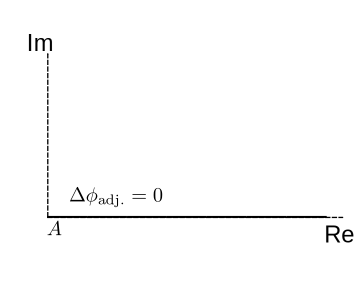
\includegraphics[width=2.5in]{phasors/manySlitPhasorsMax}
\end{center}
\caption{\label{manySlitPhasorsMaxFig}Phasor diagram for the maximum of the
single-slit diffraction pattern.}
\end{figure}




%\noindent\textbf{Example:} 
\begin{example}{Minimum of Single-Slit Diffraction Pattern}
\label{exampleSingleSlit}



Light of wavelength $600\units{nm}$ illuminates a slit of
width $2\,\mu$m. Find the distance between the central maximum and the
neighboring minimum on a screen $1.5\units{m}$ away.

%\noindent\textbf{Solution:} 
%\solution
\begin{solution}
We want to find a minimum of the diffraction
pattern, i.e., a point at which the total amplitude goes to zero.
Then the starting point of our $N$-phasor diagram must be the same as
the ending point, so that the resultant has length zero.  How do we
make a circular arc end up where it started?  By closing the circle,
as shown in Fig.~\ref{manySlitPhasorsMinFig}.  From the diagram, we can read off the phase
difference $\Delta\phi_\text{tot}$ between the first and last
phasor--the first phasor points right, by the top of the circle it has
rotated $180^\circ$ or $\pi$\,radians to point left, and by the end,
it has rotated around to $360^\circ$ or $2\pi$\,radians.  Or, in other words,
 going in
a complete circle means rotating by
$\Delta\phi_\text{tot}=2\pi$\,radians.

Now we want to calculate where on the screen  this minimum occurs.
 From here on out, it's
the same calculation we've done with other slit patterns:
\begin{align*} 
\Delta\phi_\text{tot}=2\pi&=\frac{2\pi
a}{\lambda}\sin\theta\\ 
%2\pi&=\frac{2\pi a}{\lambda}\sin\theta\\
\lambda &= a\sin\theta\\
600\times 10^{-9}\,\text{m} &= 2\times 10^{-6}\,\text{m} \sin\theta\\
%0.2&=\sin\theta\\
\theta&=\arcsin \left(
\frac{6\times 10^{-7}}{2\times 10^{-6}} \right)
=  \arcsin \left(0.3\right) = 0.305\,\text{rad}
\end{align*}
Now, by the geometry of the right triangle formed by the line
to the minimum on the screen, the line to the central maximum, and the screen itself, we can calculate the desired distance on the screen:
\begin{align*}
y &= L \tan\theta \\ 
y&=1.5\,\text{m} \tan\left( 0.305 
\right)= \fbox{\,\,0.472\,m\phantom{\Big (}}
\end{align*}
\end{solution}
\end{example}

\begin{figure}[t]
\begin{center}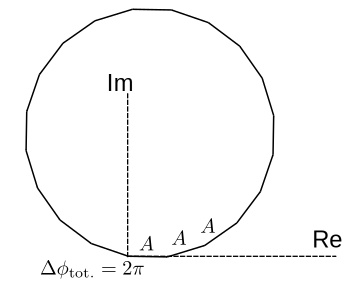
\includegraphics[width=2.in]{phasors/manySlitPhasorsMin}
\end{center}
\caption{\label{manySlitPhasorsMinFig}Phasor diagram for a minimum of the
single-slit diffraction pattern.}
\end{figure}

\begin{figure}[b]
\begin{center}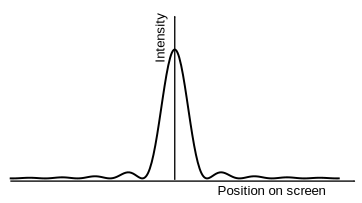
\includegraphics[width=2.9in]{phasors/singleSlitPattern}
\end{center}
\caption{\label{singleSlitFig}Single-slit diffraction pattern.}
\end{figure}





\section{Diffraction Limit}
\label{sec:diffraction_limit}

We can learn a lot from the single slit. As seen in Example \ref{exampleSingleSlit},
the first minimum of the single-slit pattern happens when
$\Delta\phi_\text{tot}= 2\pi$ or
$\lambda = a\sin\theta$.  In many cases, the wavelength $\lambda$ is substantially
smaller than the size of the slit, and we can safely use the small-angle approximation
$\sin\theta\approx\theta$.  Note that $\theta$ must be in radians for this to 
be a good approximation--try it out on your calculator for some large ($\theta$
around 1 or bigger) and some small ($\theta$ much less than 1) values of $\theta$,
to convince yourself you understand how this approximation works.
In this approximation, we can then rearrange this equation:
\begin{equation}
\theta \approx \frac{\lambda}{a}
.\end{equation}
This equation is known as the \textbf{diffraction limit}.
It   doesn't look  like much,  but we can  squeeze a  lot of
useful information out of it.  First of all, it says that when we decrease 
the wavelength $\lambda$, the waves spread out (diffract) by a smaller angle 
when they pass through a  slit or aperture. Similarly, if we use a bigger slit, 
the waves also spread out less. 

Why do we care how much wave spread out when they pass through an aperture?  
Because that's how we see and hear things, and how all optical instruments like
telescopes, binoculars, and microscopes work.

\begin{example}{The Naked Eye}
\label{exampleNakedEye}
If your eye were limited solely by diffraction (i.e., your vision was perfect),
would you be able to distinguish how many fingers your friend
was holding up at a distance of $10\units{km}$? If not, how large a telescope
would you need to distinguish them?

%\solution 
\begin{solution}
Let's estimate the distance between a person's fingers as
about $\Delta x=1\units{cm}$.  The distance between you and your
friend is $L=10\units{km}$.  So the angle between your friend's two
fingers, as viewed by you, is
\begin{equation}
\theta_\text{fingers}=2\arctan\frac{\Delta
  x}{2L}=2\arctan\frac{1\units{cm}}{2\cdot 10\units{km}}\approx
10^{-6}\units{rad}.
\end{equation}
The diameter of your eye (the iris, or aperture) is around
$0.5\units{cm}$, and let's assume we're using light in the middle of
the visible spectrum, around $500\units{nm}$.  So, using the
diffraction limit equation above,
\begin{equation}
\theta_\text{diffraction}\approx \frac{500\times
  10^{-9}\units{m}}{0.5\times 10^{-2}\units{m}} =10^{-4}\units{rad}.
\end{equation}

How can we interpret this? Well, we calculated that the angle between
two light rays coming from the two adjacent fingers are only separated
by an angle of $\theta_\text{fingers}=10^{-6}\units{rad}$, but when
they pass through they aperture of the eye, they diffract and are
smeared out over an angle of about
$\theta_\text{diffraction}=10^{-4}\units{rad}$.  As a result, the
light from the two fingers is smeared into one large blurry blob, and
you have no hope of distinguishing the two fingers.  (In fact, you can
do the calculation and show that at a distance of $10\units{km}$,
you'd be unable to distinguish any two objects closer than about a
meter with the naked eye.)

What if we had a telescope? Then we'd effectively be able to make the
diameter of the aperture bigger.  How much bigger would $a$ have to be
for you to see your friends fingers?  Well, our diffraction angle was
a factor of 100 bigger than the angular separation of the fingers. So
we'd have to drop $\theta_\text{diffraction}$ by a factor of 100.  If
we're not going to change $\lambda$, we'll have to increase the
aperture by a factor of 100, which means using a telescope of diameter
$a_\text{telescope} = 100a_\text{eye} \approx 0.5\units{m}$.  That's a
pretty hefty telescope --- probably not one you'll want to carry around
with you!

\end{solution}
\end{example}


This example highlights the  concept of \textbf{resolution}, which you
may have  encountered in other contexts, like  photography or computer
monitors. A  high-resolution image  is a very  crisp, clear  one, with
minimal      blurring.      Since      the     two      fingers     in
Example~\ref{exampleNakedEye} were blurred together by diffraction, we
say that they were not resolved. 

Since  blurring is a  fairly fuzzy  concept, we  usually won't  try to
distinguish exactly when  two objects go from being  resolved to being
unresolved. Mostly we'll be interested just in whether they're clearly
resolved or not.   As a side note, though, there  is a clear criterion
called Rayleigh's criterion that's sometimes used to state whether two
objects are resolved or not.  Rayleigh's criterion for determining the
cutoff when two  objects go from being resolved  to unresolved is that
when the maximum of one object's diffraction pattern lines up with the
minimum of the  other's diffraction pattern, then the  objects go from
being resolved to being unresolved.

The diffraction limit helps  us understand many practical applications
of waves.  We've focused on  making the aperture larger or smaller for
light waves, but  another option is to make  $\lambda$ smaller, either
by using  blue or ultraviolet light  or by switching  to electrons. It
turns  out,  as  we'll  see  when we  study  quantum  mechanics,  that
electrons  also  have  a  wavelength,  and for  typical  energies  the
electron wavelength is much  shorter than an optical wavelength.  Thus
using electrons  to image small  objects can produce images  with much
higher resolution than is achievable  with light. This is the fundamental
principle behind
the  electron microscope.   Going to  shorter wavelengths  (and higher
frequencies)  is also  the basis  of medical  ultrasound measurements,
which  use  very high-frequency  sound  waves  to  probe the  internal
structure of  the human body. Using regular  low-frequency sound waves
would  result extremely  blurry  images, since  the diffraction  angle
would be large.



% Note that but current-generation astronomical telescopes have diameters around
% 10\,m, and plans are in the works for telescopes  with diameters of around 30\,m!
% Such large diameters help


\begin{figure}
\begin{center}
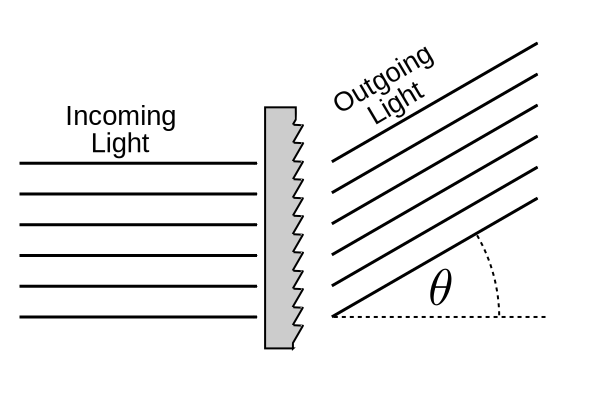
\includegraphics[width=2.5in]{phasors/grating}
\end{center}
\caption{\label{fig:grating}Light incident on a diffraction grating.}
\end{figure}



\section{Diffraction Gratings}
\label{sec:diffraction_gratings}

A  diffraction grating  consists of  many very  small,  equally spaced
slits. A grating can be either a transmission grating (as pictured
in Fig.~\ref{fig:grating}, where the light
comes from one side and gets diffracted out the other, or a reflection
grating, where the light gets diffracted  back on the same side of the
grating that it came from.  The ``slits'' may consist of absorbing and
transparent regions, as with our double and triple slits, or simply of
ridges in  a transparent material,  or of angled  reflecting surfaces.
Historically,   the   first   diffraction   gratings  were   made   by
painstakingly  etching thousands  of microscopic  parallel  grooves in
glass using a diamond scribe.  Fortunately, the details of how the
grooves, lines, or slits are shaped doesn't affect where the light gets diffracted. (It does affect how \emph{much} light gets diffracted, but we won't worry about calculating that.) 

Everything  we  did  for  two  and  three  slits  carries  over  to  a
diffraction grating,  except that now we  have a very  large number of
phasors (in the  range of 1000 to 10,000). That  means we can't easily
draw them  all and add  them as vectors,  but we can still  figure out
what the diffraction pattern must look like. 


\begin{figure}
\begin{center}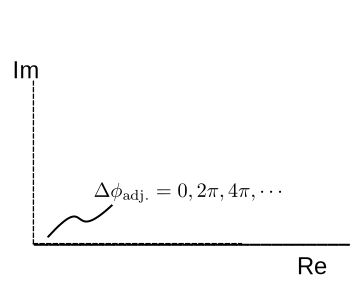
\includegraphics[width=2.4in]{phasors/gratingPhasorMax}
\end{center}
\caption{\label{gratingMaxFig}Phasor diagram for a diffraction grating
at a maximum of the intensity.}
\end{figure}


Suppose our grating is illuminated at normal incidence by light of
wavelength $\lambda$, so that the light reaches all the slits in
phase.  Each slit re-radiates its own outgoing wave, and these waves
interfere on a distant screen. We represent each interfering wave as
a phasor on a phasor diagram.  To get a maximum from our many-phasor
diagram, we want all the phasors pointing in the same direction, as
in Fig.~\ref{gratingMaxFig}.  This happens when the phase difference
between two adjacent phasors is $0$, but also when it is $2\pi$, $4\pi$,
etc., and when it is $-2\pi$, $-4\pi$, etc.  Thus we have maxima in the
intensity for any integer multiple of $2\pi$, provided the angle of the
outgoing light is small enough that the light can actually reach the
screen. These maxima are often referred to as ``orders'' of diffraction,
where $\Delta\phi=0$ is called the zeroth order, $\Delta\phi=2\pi$ is the
first order, $\Delta\phi = 4\pi$ is the second order, $\Delta\phi=-2\pi$
the minus-first order, etc.

\begin{figure}[b]
\begin{center}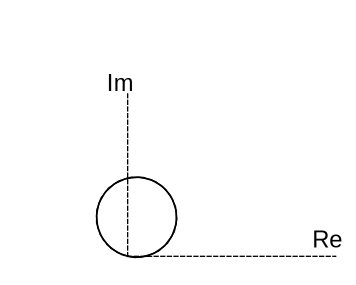
\includegraphics[width=2.4in]{phasors/gratingPhasorNonMax}
\end{center}
\caption{\label{gratingNonMaxFig}Phasor diagram for a diffraction grating
away from a maximum.}
\end{figure}

What about points on the screen that \emph{aren't} maxima?  If we move
away from  the central maximum by  a small distance,  there's now some
non-zero  phase difference  $\Delta\phi_\text{adj.}$. This  means that
each adjacent  phasor is rotated  by $\Delta\phi_\text{adj.}$ relative
to its neighbor. But remember, we now have A LOT of phasors. So the by
the time we've  gotten through our 1000 or  10,000 phasors, the phasor
diagram  has  wrapped itself  up  in  a tight little  circles,  as
indicated in  Fig.~\ref{gratingNonMaxFig}. The  amplitude won't be  exactly zero,  but it
will  be  much  less  than  the  amplitude at  the  maximum.  And  the
intensity, which  is proportional to amplitude squared,  will be MUCH,
MUCH less  than at the maximum.   This is why  the diffraction pattern
from the grating  consists of very narrow maxima,  where all the light
is  concentrated, and wide  expanses in  between where  essentially no
light goes.   (Incidentally, you can  see from conservation  of energy
that  when  the  maxima get  very  bright,  they  must also  get  very
narrow--otherwise the  total light power reaching the  screen would be
bigger than the light power passing through the slit!)

You can think  of the grating diffraction pattern as  the limit of the
$N$-slit    pattern,    when   $N$    gets    big.    As   shown    in
Fig.~\ref{gratingSlitPatterns}, the  primary maxima of  the multi-slit
pattern get  narrower and  narrower as the  number of  slits increases
(assuming a constant slit  spacing).  These maxima get correspondingly
brighter, since if  the amplitude from each slit  is $A$, the combined
amplitude  from $N$  slits at  a maximum  is $N  A$, and  the combined
intensity is  proportional to  $N^2 A^2$, which  grows rapidly  as the
number of slits increases.


\begin{figure}
\begin{center}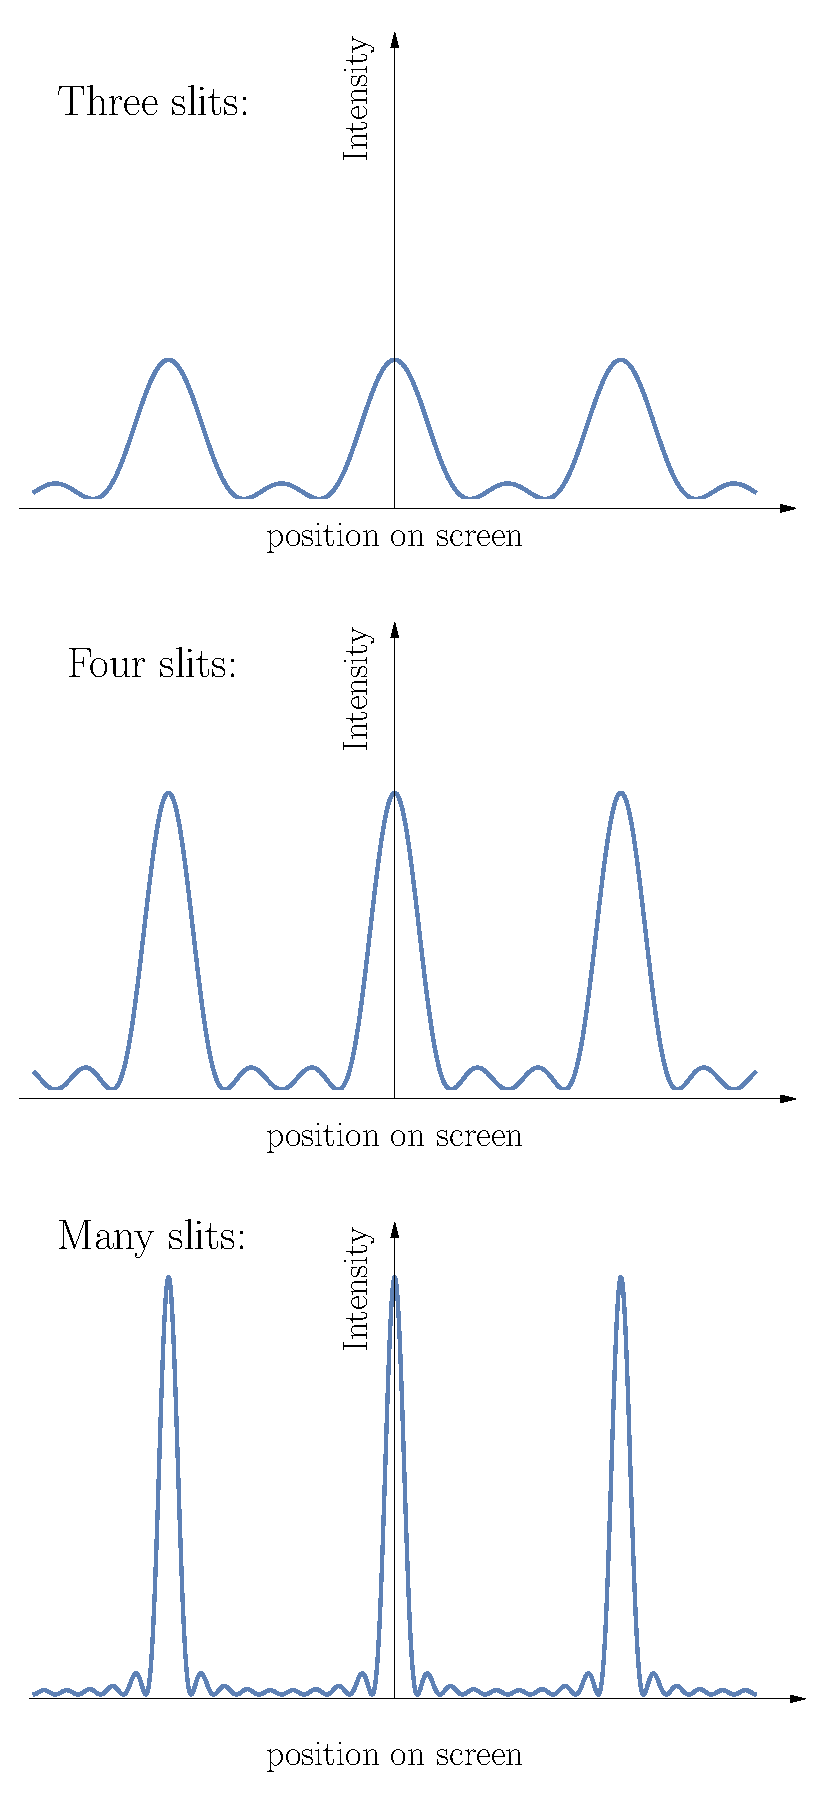
\includegraphics[width=2.7in]{phasors/gratingSlitPatterns}
\end{center}
\caption{\label{gratingSlitPatterns} The diffraction pattern of multiple
slits begins to resemble that of a diffraction grating as the number of 
slits increases, with very narrow, very bright peaks.}
\end{figure}

% \begin{figure}
% \begin{center}
% 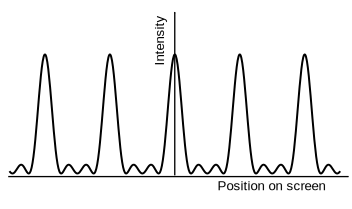
\includegraphics[width=10cm]{phasors/fourSlitPattern}  
% \end{center}
% \caption{\label{fourSlitFig}Four-slit pattern.}
% \end{figure}

% \begin{figure}
% \begin{center}
% 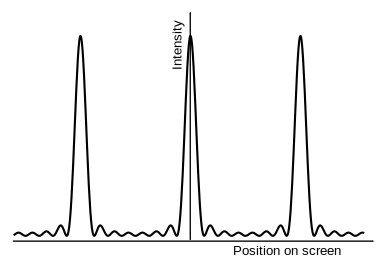
\includegraphics[width=10cm]{phasors/gratingPattern}  
% \end{center}
% \caption{\label{gratingPatternFig} The many-slit pattern begins to approach
% the appearance of a diffraction-grating pattern: bright spots, with very 
% little diffraction in between.}
% \end{figure}



%\section{Huyghens' Principle?}





\newpage


\section*{Problems}
\label{sec:phasors_problems}
\markright{PROBLEMS}


\begin{problem}
Draw phasor diagrams depicting the oscillations described below at the noted times:
  \begin{enumerate}
  \item For the oscillation $x(t) = 3\cos\left(\frac{\pi}{3}t\right)$, draw
phasor diagrams for $t = 0$, 1, 2, 3, 5, and $6\units{s}$.
  \item For the oscillation 
 \[ x(t) = 3e^{i\left(\frac{\pi}{3}t + \frac{\pi}{3}\right)} \]
draw complex phasor diagrams for $t = 0$, 1, 2, 3, 5, and $6\units{s}$.
  \end{enumerate}
\end{problem}


\begin{problem}
Consider water waves passing by a fixed point with a period  
of $6\units{s}$ and a height $30\units{cm}$. Imagine 
that $t=0$ corresponds to the moment when the water surface returns 
to its equilibrium position just after a crest passes.
  \begin{enumerate}
  \item Draw phasor diagrams for the displacement of the water for times 
$t = 0, 1, 2, 3, 5$, and $6\units{s}$.
  \item Write an expression for this oscillation in the form
\[ x(t) = Ae^{i\left(\omega t + \phi_0\right)}   \]
specifying $A$, $\omega$, and $\phi_0$.
  \end{enumerate}
\label{prob:waterwaves}
\end{problem}

\begin{problem}
Draw a phasor diagram describing these oscillations:
\begin{enumerate}
\item $\displaystyle\hspace{0.1in}x(t) = 4 \cos\left(\frac{\pi}{4}t 
+ \frac{\pi}{2}\right) \hspace{0.2in} \mbox{at time $t=3\units{s}$}$
\vspace{0.1in}

\item $\displaystyle\hspace{0.1in}x(t) = 4 e^{i\left(\frac{\pi}{2} 
- \frac{\pi}{4}t\right)} \hspace{0.2in} \mbox{at time $t=3\units{s}$}$
\end{enumerate}
\end{problem}

\begin{problem}
Write the superposition of the following two oscillations
\[ 
x_1(t) = 3\cos\left(\frac{\pi}{4}t\right)\quad\quad
 x_2(t) = 5\cos\left(\frac{\pi}{4}t + \frac{\pi}{3}\right) 
\]
in the form
\[ 
x_3(t) = A_3 \cos\left(\omega t + \phi_3\right) 
\]
and determine $A_3$ and $\phi_3$.  (Hint: Use phasor addition!)
\end{problem}

\newpage

\begin{problem}
You're standing at the point $P$ on a line between two radio towers, 
A and B. 

 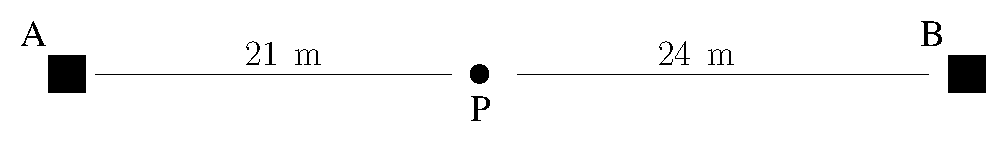
\includegraphics[width=4.0truein]{phasors/phasor26} 

\noindent Both towers broadcast the same radio signal of wavelength $\lambda =
12\units{m}$. With only tower A broadcasting, you measure a wave amplitude
of 6 (in some unspecified unit).  With only tower B broadcasting, you
measure a wave amplitude of 3. What amplitude do you measure when both
towers are broadcasting?
\label{prob:between_towers}
\end{problem}


\begin{problem}
You're sitting in the Weis Center listening to the 
``Sonorous Symphony in C,'' which consists of
a single 128 Hz tone played through two speakers separated by
$5\units{m}$ on stage. Both speakers emit sound waves in phase.

 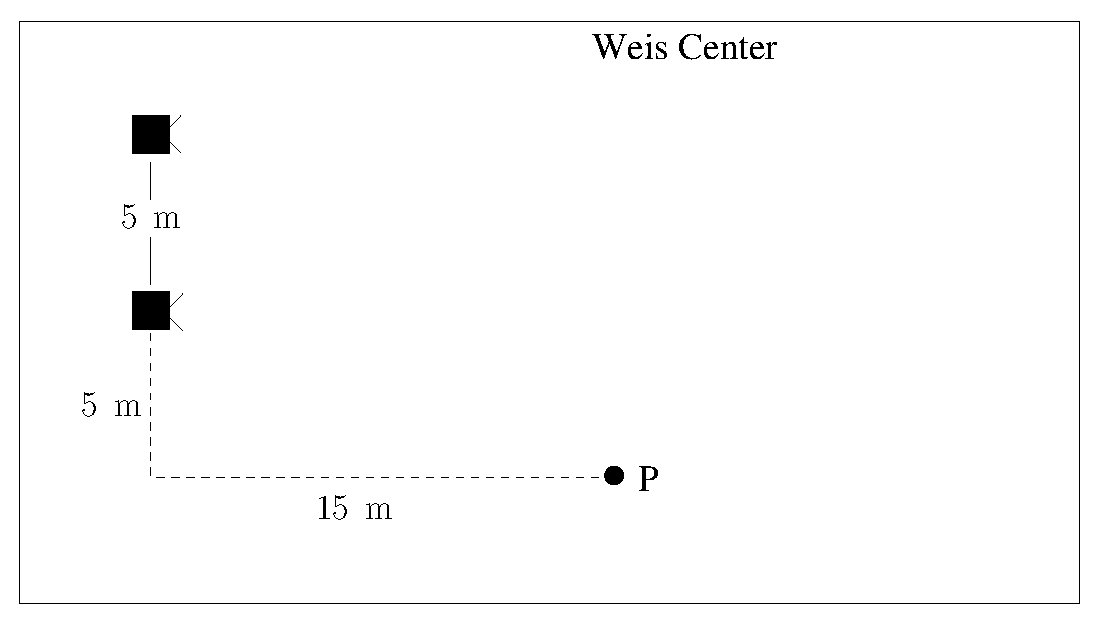
\includegraphics[width=4.0truein]{phasors/phasor14} 

\noindent You happen to be sitting at the point $P$ in the above
diagram, $5\units{m}$ to the left of the leftmost speaker, and
$15\units{m}$ back from the stage.

If the wave amplitude at your location from each speaker individually
is $A$, what is the amplitude of the combined waves from both speakers
at your location?
\end{problem}

\newpage

\begin{problem}
Three radio towers, arrayed as indicated in the figure, each broadcast
the same in-phase signal with wavelength $\lambda = 5\units{m}$.

 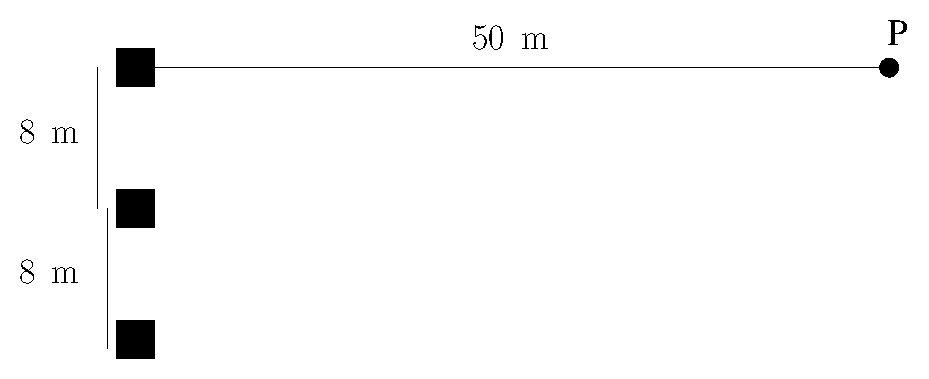
\includegraphics[width=2.4truein]{phasors/phasor25} 

\noindent If the amplitude from each tower individually at point $P$
is $A$, what is the amplitude of the combined signal from the three
towers?

\noindent ({\em Hint:} $d\sin{\theta}$ won't work here. Calculate 
the distances and figure out the path length differences directly.)
\label{prob:three_towers}
\end{problem}

\begin{problem}
Light of wavelength $\lambda = 617\units{nm}$ passes
through a three-slit system where the slits are separated by a
distance $d = 1.4 \times 10^{-5}\units{m}$, and produces an
interference pattern on a distant screen. Determine the amplitude of the 
light directed at an angle $\theta = 0.23^\circ$ from the direction to 
the central maximum in the interference pattern. Assume that the amplitude 
of the light from each slit individually is $A$.
%%%% Answer: 2.67A %%%
\end{problem}

\begin{problem}
Light of wavelength $\lambda = 532\units{nm}$ passes
through a four-slit system where the slits are separated by a
distance $d = 1.7 \times 10^{-5}\units{m}$, and produces an
interference pattern on a distant screen.
\begin{enumerate}
\item  Draw phasor diagrams for the {\em three} minima between the central
maximum and the first side maximum in the interference pattern, and
determine the values of $\Delta\phi$ for each situation.
\item Calculate the angles (relative to the direction to the central
maximum) where each of these minima occurs.
\end{enumerate}
\label{prob:four_slits}
\end{problem}

\begin{problem}
  Light of  wavelength $600\units{nm}$ is  incident normally on a grating  with $850$
  lines per millimeter. The diffraction pattern is observed on a distant screen.
\begin{enumerate}

\item  Sketch a  phasor  diagram  for the  light  at the  second-order
  maximum of the  diffraction pattern.  Be sure to  indicate the phase
  difference between  adjacent phasors on your  diagram.  (Don't worry
  about  the   fact  that  you   can't  draw  all  the   thousands  of
  phasors--just draw 5 or 6 representative phasors.)

\item Using your phasor diagram and the adjacent phase difference you determined
in part (a), find the angle to the normal at which the second-order diffraction
maximum occurs.
\end{enumerate}
\end{problem}


\begin{problem}
 Sodium   has  two   emission   lines  with
  $\lambda_1=589.00\units{nm}$and  $\lambda_2=589.59\units{nm}$.   
You  send light
made up of both wavelengths through a transmission grating with $1000$ lines
per millimeter and onto a screen one meter distant.  By what distance
will the first-order bright spots formed by the two wavelengths be separated?
\end{problem}

\begin{problem}
  You wish  to design a spectrometer, using  a transmission diffraction
  grating to spread light of different wavelengths out horizontally
for observation on a
distant screen.
Your design specifications state  that 
the second-order diffracted light must all fit on a
  screen $1.3\units{m}$  away and $1.7\units{m}$ wide, with the zero-order light hitting
the center of the screen.  The wavelengths  you intend to  analyze with
  the spectrometer fall between $450\units{nm}$ and $800\units{nm}$.
%
\begin{enumerate}

\item Determine the maximum  allowed number of lines per millimeter
for the grating.
\item Using your answer for part (a), determine whether or not  the first and second-order bands of diffracted light will overlap.
\end{enumerate}
\end{problem}

\begin{problem}
Light of wavelength $500\units{nm}$ illuminates a single slit of width
$5\units{$\mu$m}$. At the center of the diffraction pattern on a  screen $1\units{m}$
away, the amplitude of the light is $A$. Determine the amplitude 
of the light
on the screen a distance of $2.5\units{cm}$ away from the center of the central maximum.
\end{problem}




\begin{problem}
  A  telescope  is  being   designed  to  detect  distant  binary-star
  systems. The telescope should be able to detect stars separated by 
   $10^{-4}\units{lt-yr}$ at  a distance of $300\units{lt-yr}$, using
  near  infrared light  of wavelength  $1\units{$\mu$m}$.   Approximately what
minimum  diameter should the telescope have, if its performance is limited
by diffraction?
\end{problem}



